
%% bare_conf.tex
%% V1.3
%% 2007/01/11
%% by Michael Shell
%% See:
%% http://www.michaelshell.org/
%% for current contact information.
%%
%% This is a skeleton file demonstrating the use of IEEEtran.cls
%% (requires IEEEtran.cls version 1.7 or later) with an IEEE conference paper.
%%
%% Support sites:
%% http://www.michaelshell.org/tex/ieeetran/
%% http://www.ctan.org/tex-archive/macros/latex/contrib/IEEEtran/
%% and
%% http://www.ieee.org/

%%*************************************************************************
%% Legal Notice:
%% This code is offered as-is without any warranty either expressed or
%% implied; without even the implied warranty of MERCHANTABILITY or
%% FITNESS FOR A PARTICULAR PURPOSE! 
%% User assumes all risk.
%% In no event shall IEEE or any contributor to this code be liable for
%% any damages or losses, including, but not limited to, incidental,
%% consequential, or any other damages, resulting from the use or misuse
%% of any information contained here.
%%
%% All comments are the opinions of their respective authors and are not
%% necessarily endorsed by the IEEE.
%%
%% This work is distributed under the LaTeX Project Public License (LPPL)
%% ( http://www.latex-project.org/ ) version 1.3, and may be freely used,
%% distributed and modified. A copy of the LPPL, version 1.3, is included
%% in the base LaTeX documentation of all distributions of LaTeX released
%% 2003/12/01 or later.
%% Retain all contribution notices and credits.
%% ** Modified files should be clearly indicated as such, including  **
%% ** renaming them and changing author support contact information. **
%%
%% File list of work: IEEEtran.cls, IEEEtran_HOWTO.pdf, bare_adv.tex,
%%                    bare_conf.tex, bare_jrnl.tex, bare_jrnl_compsoc.tex
%%*************************************************************************

% *** Authors should verify (and, if needed, correct) their LaTeX system  ***
% *** with the testflow diagnostic prior to trusting their LaTeX platform ***
% *** with production work. IEEE's font choices can trigger bugs that do  ***
% *** not appear when using other class files.                            ***
% The testflow support page is at:
% http://www.michaelshell.org/tex/testflow/



% Note that the a4paper option is mainly intended so that authors in
% countries using A4 can easily print to A4 and see how their papers will
% look in print - the typesetting of the document will not typically be
% affected with changes in paper size (but the bottom and side margins will).
% Use the testflow package mentioned above to verify correct handling of
% both paper sizes by the user's LaTeX system.
%
% Also note that the "draftcls" or "draftclsnofoot", not "draft", option
% should be used if it is desired that the figures are to be displayed in
% draft mode.
%
\documentclass[conference]{IEEEtran}
\usepackage{blindtext, graphicx}
% Add the compsoc option for Computer Society conferences.
%
% If IEEEtran.cls has not been installed into the LaTeX system files,
% manually specify the path to it like:
% \documentclass[conference]{../sty/IEEEtran}




% Some very useful LaTeX packages include:
% (uncomment the ones you want to load)


% *** MISC UTILITY PACKAGES ***
%
%\usepackage{ifpdf}
% Heiko Oberdiek's ifpdf.sty is very useful if you need conditional
% compilation based on whether the output is pdf or dvi.
% usage:
% \ifpdf
%   % pdf code
% \else
%   % dvi code
% \fi
% The latest version of ifpdf.sty can be obtained from:
% http://www.ctan.org/tex-archive/macros/latex/contrib/oberdiek/
% Also, note that IEEEtran.cls V1.7 and later provides a builtin
% \ifCLASSINFOpdf conditional that works the same way.
% When switching from latex to pdflatex and vice-versa, the compiler may
% have to be run twice to clear warning/error messages.






% *** CITATION PACKAGES ***
%
%\usepackage{cite}
% cite.sty was written by Donald Arseneau
% V1.6 and later of IEEEtran pre-defines the format of the cite.sty package
% \cite{} output to follow that of IEEE. Loading the cite package will
% result in citation numbers being automatically sorted and properly
% "compressed/ranged". e.g., [1], [9], [2], [7], [5], [6] without using
% cite.sty will become [1], [2], [5]--[7], [9] using cite.sty. cite.sty's
% \cite will automatically add leading space, if needed. Use cite.sty's
% noadjust option (cite.sty V3.8 and later) if you want to turn this off.
% cite.sty is already installed on most LaTeX systems. Be sure and use
% version 4.0 (2003-05-27) and later if using hyperref.sty. cite.sty does
% not currently provide for hyperlinked citations.
% The latest version can be obtained at:
% http://www.ctan.org/tex-archive/macros/latex/contrib/cite/
% The documentation is contained in the cite.sty file itself.






% *** GRAPHICS RELATED PACKAGES ***
%
\ifCLASSINFOpdf
  % \usepackage[pdftex]{graphicx}
  % declare the path(s) where your graphic files are
  % \graphicspath{{../pdf/}{../jpeg/}}
  % and their extensions so you won't have to specify these with
  % every instance of \includegraphics
  % \DeclareGraphicsExtensions{.pdf,.jpeg,.png}
\else
  % or other class option (dvipsone, dvipdf, if not using dvips). graphicx
  % will default to the driver specified in the system graphics.cfg if no
  % driver is specified.
  % \usepackage[dvips]{graphicx}
  % declare the path(s) where your graphic files are
  % \graphicspath{{../eps/}}
  % and their extensions so you won't have to specify these with
  % every instance of \includegraphics
  % \DeclareGraphicsExtensions{.eps}
\fi
% graphicx was written by David Carlisle and Sebastian Rahtz. It is
% required if you want graphics, photos, etc. graphicx.sty is already
% installed on most LaTeX systems. The latest version and documentation can
% be obtained at: 
% http://www.ctan.org/tex-archive/macros/latex/required/graphics/
% Another good source of documentation is "Using Imported Graphics in
% LaTeX2e" by Keith Reckdahl which can be found as epslatex.ps or
% epslatex.pdf at: http://www.ctan.org/tex-archive/info/
%
% latex, and pdflatex in dvi mode, support graphics in encapsulated
% postscript (.eps) format. pdflatex in pdf mode supports graphics
% in .pdf, .jpeg, .png and .mps (metapost) formats. Users should ensure
% that all non-photo figures use a vector format (.eps, .pdf, .mps) and
% not a bitmapped formats (.jpeg, .png). IEEE frowns on bitmapped formats
% which can result in "jaggedy"/blurry rendering of lines and letters as
% well as large increases in file sizes.
%
% You can find documentation about the pdfTeX application at:
% http://www.tug.org/applications/pdftex





% *** MATH PACKAGES ***
%
%\usepackage[cmex10]{amsmath}
% A popular package from the American Mathematical Society that provides
% many useful and powerful commands for dealing with mathematics. If using
% it, be sure to load this package with the cmex10 option to ensure that
% only type 1 fonts will utilized at all point sizes. Without this option,
% it is possible that some math symbols, particularly those within
% footnotes, will be rendered in bitmap form which will result in a
% document that can not be IEEE Xplore compliant!
%
% Also, note that the amsmath package sets \interdisplaylinepenalty to 10000
% thus preventing page breaks from occurring within multiline equations. Use:
%\interdisplaylinepenalty=2500
% after loading amsmath to restore such page breaks as IEEEtran.cls normally
% does. amsmath.sty is already installed on most LaTeX systems. The latest
% version and documentation can be obtained at:
% http://www.ctan.org/tex-archive/macros/latex/required/amslatex/math/





% *** SPECIALIZED LIST PACKAGES ***
%
%\usepackage{algorithmic}
% algorithmic.sty was written by Peter Williams and Rogerio Brito.
% This package provides an algorithmic environment fo describing algorithms.
% You can use the algorithmic environment in-text or within a figure
% environment to provide for a floating algorithm. Do NOT use the algorithm
% floating environment provided by algorithm.sty (by the same authors) or
% algorithm2e.sty (by Christophe Fiorio) as IEEE does not use dedicated
% algorithm float types and packages that provide these will not provide
% correct IEEE style captions. The latest version and documentation of
% algorithmic.sty can be obtained at:
% http://www.ctan.org/tex-archive/macros/latex/contrib/algorithms/
% There is also a support site at:
% http://algorithms.berlios.de/index.html
% Also of interest may be the (relatively newer and more customizable)
% algorithmicx.sty package by Szasz Janos:
% http://www.ctan.org/tex-archive/macros/latex/contrib/algorithmicx/




% *** ALIGNMENT PACKAGES ***
%
%\usepackage{array}
% Frank Mittelbach's and David Carlisle's array.sty patches and improves
% the standard LaTeX2e array and tabular environments to provide better
% appearance and additional user controls. As the default LaTeX2e table
% generation code is lacking to the point of almost being broken with
% respect to the quality of the end results, all users are strongly
% advised to use an enhanced (at the very least that provided by array.sty)
% set of table tools. array.sty is already installed on most systems. The
% latest version and documentation can be obtained at:
% http://www.ctan.org/tex-archive/macros/latex/required/tools/


%\usepackage{mdwmath}
%\usepackage{mdwtab}
% Also highly recommended is Mark Wooding's extremely powerful MDW tools,
% especially mdwmath.sty and mdwtab.sty which are used to format equations
% and tables, respectively. The MDWtools set is already installed on most
% LaTeX systems. The lastest version and documentation is available at:
% http://www.ctan.org/tex-archive/macros/latex/contrib/mdwtools/


% IEEEtran contains the IEEEeqnarray family of commands that can be used to
% generate multiline equations as well as matrices, tables, etc., of high
% quality.


%\usepackage{eqparbox}
% Also of notable interest is Scott Pakin's eqparbox package for creating
% (automatically sized) equal width boxes - aka "natural width parboxes".
% Available at:
% http://www.ctan.org/tex-archive/macros/latex/contrib/eqparbox/





% *** SUBFIGURE PACKAGES ***
%\usepackage[tight,footnotesize]{subfigure}
% subfigure.sty was written by Steven Douglas Cochran. This package makes it
% easy to put subfigures in your figures. e.g., "Figure 1a and 1b". For IEEE
% work, it is a good idea to load it with the tight package option to reduce
% the amount of white space around the subfigures. subfigure.sty is already
% installed on most LaTeX systems. The latest version and documentation can
% be obtained at:
% http://www.ctan.org/tex-archive/obsolete/macros/latex/contrib/subfigure/
% subfigure.sty has been superceeded by subfig.sty.



%\usepackage[caption=false]{caption}
%\usepackage[font=footnotesize]{subfig}
% subfig.sty, also written by Steven Douglas Cochran, is the modern
% replacement for subfigure.sty. However, subfig.sty requires and
% automatically loads Axel Sommerfeldt's caption.sty which will override
% IEEEtran.cls handling of captions and this will result in nonIEEE style
% figure/table captions. To prevent this problem, be sure and preload
% caption.sty with its "caption=false" package option. This is will preserve
% IEEEtran.cls handing of captions. Version 1.3 (2005/06/28) and later 
% (recommended due to many improvements over 1.2) of subfig.sty supports
% the caption=false option directly:
%\usepackage[caption=false,font=footnotesize]{subfig}
%
% The latest version and documentation can be obtained at:
% http://www.ctan.org/tex-archive/macros/latex/contrib/subfig/
% The latest version and documentation of caption.sty can be obtained at:
% http://www.ctan.org/tex-archive/macros/latex/contrib/caption/




% *** FLOAT PACKAGES ***
%
%\usepackage{fixltx2e}
% fixltx2e, the successor to the earlier fix2col.sty, was written by
% Frank Mittelbach and David Carlisle. This package corrects a few problems
% in the LaTeX2e kernel, the most notable of which is that in current
% LaTeX2e releases, the ordering of single and double column floats is not
% guaranteed to be preserved. Thus, an unpatched LaTeX2e can allow a
% single column figure to be placed prior to an earlier double column
% figure. The latest version and documentation can be found at:
% http://www.ctan.org/tex-archive/macros/latex/base/



%\usepackage{stfloats}
% stfloats.sty was written by Sigitas Tolusis. This package gives LaTeX2e
% the ability to do double column floats at the bottom of the page as well
% as the top. (e.g., "\begin{figure*}[!b]" is not normally possible in
% LaTeX2e). It also provides a command:
%\fnbelowfloat
% to enable the placement of footnotes below bottom floats (the standard
% LaTeX2e kernel puts them above bottom floats). This is an invasive package
% which rewrites many portions of the LaTeX2e float routines. It may not work
% with other packages that modify the LaTeX2e float routines. The latest
% version and documentation can be obtained at:
% http://www.ctan.org/tex-archive/macros/latex/contrib/sttools/
% Documentation is contained in the stfloats.sty comments as well as in the
% presfull.pdf file. Do not use the stfloats baselinefloat ability as IEEE
% does not allow \baselineskip to stretch. Authors submitting work to the
% IEEE should note that IEEE rarely uses double column equations and
% that authors should try to avoid such use. Do not be tempted to use the
% cuted.sty or midfloat.sty packages (also by Sigitas Tolusis) as IEEE does
% not format its papers in such ways.





% *** PDF, URL AND HYPERLINK PACKAGES ***
%
%\usepackage{url}
% url.sty was written by Donald Arseneau. It provides better support for
% handling and breaking URLs. url.sty is already installed on most LaTeX
% systems. The latest version can be obtained at:
% http://www.ctan.org/tex-archive/macros/latex/contrib/misc/
% Read the url.sty source comments for usage information. Basically,
% \url{my_url_here}.

\usepackage{hyperref}

\usepackage{todonotes}

\usepackage{caption}
\usepackage{subcaption}



% *** Do not adjust lengths that control margins, column widths, etc. ***
% *** Do not use packages that alter fonts (such as pslatex).         ***
% There should be no need to do such things with IEEEtran.cls V1.6 and later.
% (Unless specifically asked to do so by the journal or conference you plan
% to submit to, of course. )


% correct bad hyphenation here
\hyphenation{op-tical net-works semi-conduc-tor}


\begin{document}
%
% paper title
% can use linebreaks \\ within to get better formatting as desired
\title{Touch-enabled HTML5 client for Spotify}


% author names and affiliations
% use a multiple column layout for up to three different
% affiliations
\author{\IEEEauthorblockN{Antti Partanen}
\IEEEauthorblockA{
Student number: 295967\\
\texttt{antti.partanen@aalto.fi}}
\and
\IEEEauthorblockN{Ilari Meuronen}
\IEEEauthorblockA{
Student number: 84331L\\
\texttt{ilari.meuronen@aalto.fi}}
\and
\IEEEauthorblockN{Samuli Vuorinen}
\IEEEauthorblockA{
Student number: 78771U\\
\texttt{samuli.vuorinen@aalto.fi}}}





% make the title area
\maketitle


\begin{abstract}
%\boldmath
As mobile devices are an increasingly common way of using the internet, the need for
mobile optimized web services has risen. Typical web applications are clumsy at best
compared to native applications, and get worse the more complex the application gets.
One way to reduce this gap between mobile web and native applications is to enable
touch gestures.
\todo[inline]{Abstrakti on nyt suoraan Research Planista, vaatii muutoksia. Kannattanee kirjoittaa vasta lopuksi.}

\end{abstract}
% IEEEtran.cls defaults to using nonbold math in the Abstract.
% This preserves the distinction between vectors and scalars. However,
% if the journal you are submitting to favors bold math in the abstract,
% then you can use LaTeX's standard command \boldmath at the very start
% of the abstract to achieve this. Many IEEE journals frown on math
% in the abstract anyway.

% Note that keywords are not normally used for peerreview papers.
\begin{IEEEkeywords}
HTML, Touch, Javascript, Spotify.
\end{IEEEkeywords}


% For peer review papers, you can put extra information on the cover
% page as needed:
% \ifCLASSOPTIONpeerreview
% \begin{center} \bfseries EDICS Category: 3-BBND \end{center}
% \fi
%
% For peerreview papers, this IEEEtran command inserts a page break and
% creates the second title. It will be ignored for other modes.
\IEEEpeerreviewmaketitle

\section{Introduction}

Mobile devices such as smartphones and tablets typically feature a capacitive touch screen. As mobile devices are becoming the most popular mean of accessing Internet, web developers need ways to create touch enabled and mobile friendly applications. 

Apple introduced the Touch Events API in 2007 along with the iPhone to support touch events. W3C tried to standardize Touch Events, but they ran into patent issues with Apple, so the development was stalled. Meanwhile, Microsoft developed its own Pointer Events API, intended to unify different inputs including mouse, touch and pen. 

Later, as the patent issue with Apple were not a problem for W3C anymore, Touch Events was standardized in 2013 \cite{W3CTouchEvents}. Things weren't so good for Pointer Events as chromium dropped support for it in 2014, citing performance along with other problems as an issue \url{https://code.google.com/p/chromium/issues/detail?id=162757#c64}. As a result, the browser support for Pointer Events is only backed by Microsoft's own browsers as seen in the figure below. However, in 2015 Google, along with Firefox announced their intent to support Pointer Events in Chrome in the near future. 


\begin{figure}[htbd]
    \centering
    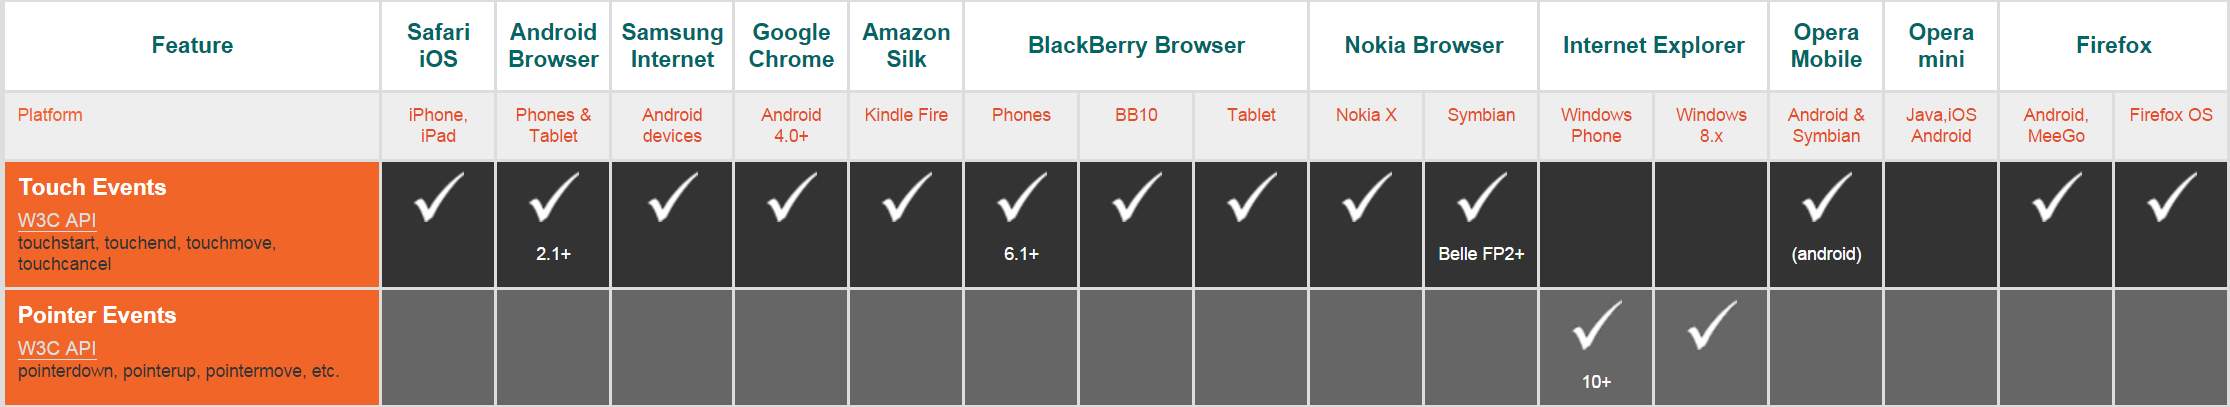
\includegraphics[scale=0.18]{htmltouchevents.png}
    \caption{Browser support for Touch Events and Pointer Events in 2015 \cite{MobileHTML5}}
\end{figure}


%Touch in browsers:
%W3C touch events, javascript libraries etc.
%Our research goals were the following:
%\begin{itemize}
%\item To explore the current status of mobile touch technologies on the web.
%\item To demonstrate the usefulness of touch gestures in web applications.
%\item To find and demonstrate the most common difficulties in developing touch-based applications.
%\item Find common usability problems and solutions for touch screens.
%\end{itemize}
%\todo[inline]{Tarkempi introduction ja ongelmakuvaus.}


In this article, we present a web application that is designed for mobile devices, implements HTML touch gestures and utilizes an external Spotify API. Our primary research goals were to explore the current status of mobile touch technologies and to find and highlight some of the most common problems and difficulties in developing touch web applications. In addition we demonstrate some practical usefulness of touch gestures.


\section{Related work}

According to Bragdon et al. direct touch gestures can produce on-par performance and accuracy compared to buttons elements. Some touch gestures can even offer significant performance gains, especially in situations with environmental distractions.
\cite{BragdonExperimental}

Since the main use case for our application is Spotify on a smartphone, it is reasonable to assume that the user might be on the go and that there are various environmental distractions present.

Billinghurst and Vu studied touch gesture usage for web browsing tasks, and found that single finger, single motion gestures
are the most natural kind of gestures for web users.
\cite{BillinghurstGestures}

Buchinger et al. implemented a touch gesture interface for a video player on a mobile device.
Their study showed that users find simple swiping and sliding gestures very intuitive on a touch screen.
However, diagonal swiping felt unintuitive for most test subjects, and should be avoided.
\cite{GestureVideoPlayer}
\todo[inline]{lissaa asioita}
\todo[inline]{Jotain juttua olemassaolevasta Spotify-applikaatiosta Androidille?}

\section{Technologies}
Interactive web applications are ubiquitous these days, and many tools and frameworks exist to get the job done.
To avoid spending time on tracking down problems and bugs in the tools we use, we opted for the most mature and stable frameworks and libraries we could find.

The project described in this report is not intended to provide a polished web application that works on every existing web browser.
Since the application is built for mobile touch screen devices, we targeted the default browser Chrome for Google Android.
Android is currently the most popular smartphone operating system, according to Gartner \cite{AndroidMarketShare}.

The development work was done using the desktop version of Google Chrome to maximize synergy with the Android equivalent. Chrome is currently the most popular web browser available \cite{W3Counter}, and it provides very good developer tools.

\subsection{Spotify API}

Spotify has developed a RESTful Spotify Web API for third-party developers \cite{SpotifyAPI}. As with any REST API, the Spotify API can be queried using HTTP and the result data is provided as JSON formatted, making it easy to use in modern HTML5 applications. Authentication in the API is handled via OAuth.

Spotify API offers an extensive access to most of Spotify's content and functionalities. It allows third-party applications to browse artists, albums, tracks and other elementary objects in the Spotify database. 

However, the most important functionality of any Spotify client, complete track playback, is not possible (as of 2015). The API only prohibits the playback of 30 second long samples. But, since our focus is on the user interface and touch gestures, and the project described in this report is merely a proof-of-concept, the lack of complete tracks is not a big issue.

\subsection{AngularJS}
The Spotify client application described in this report is built on the AngularJS web application framework \cite{AngularJS}.

AngularJS allows the user to employ any of the common MVx design patterns like Model-View-Presenter, Model-View-ViewModel or Model-View-Controller.
AngularJS calls this MVW, or Model-View-Whatever.

AngularJS was chosen due to its maturity and the wide availability of documentation, and the relative ease of prototyping new applications.

\subsection{Hammer.js}
A Javascript library called Hammer.js is responsible for handling the different touch gestures.
Hammer.js integrates well into AngularJS, is easy to use and offers a multitude of touch gesture recognizer components.
Hammer.js also supports multi-touch gestures.
\cite{HammerJS}

\section{Application user interface}
The user interface for the application was designed with the existing Spotify Android client in mind,
since that is what the users are already familiar with.
We added several touch events where they seemed fitting.

The two main views of the application are the search view and the playlist view.
They are described in more detail below.

\begin{figure}[htbp]
    \centering
    \begin{subfigure}{0.45\columnwidth}
        \centering
        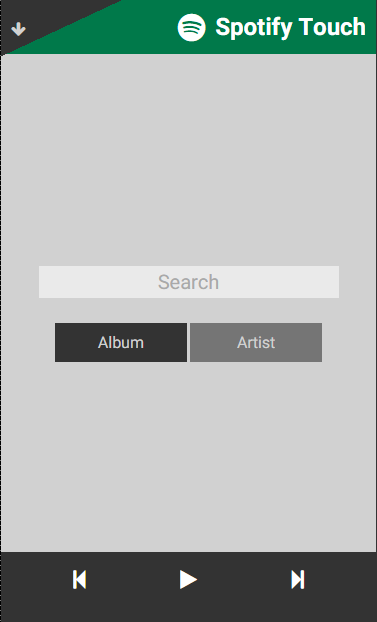
\includegraphics[width=0.9\linewidth]{spotify_search.png}
        \caption{Search view}
        \label{fig:SearchView}
    \end{subfigure}
    \begin{subfigure}{0.45\columnwidth}
        \centering
        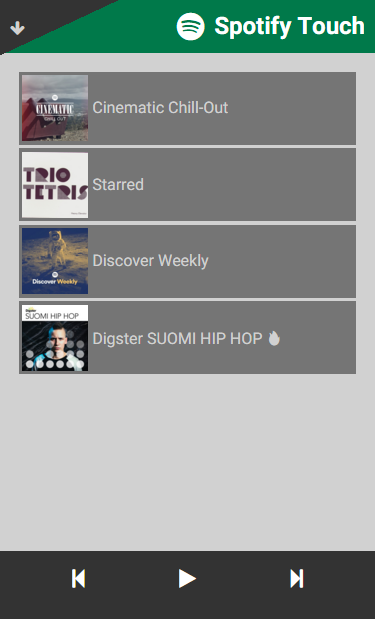
\includegraphics[width=0.9\linewidth]{spotify_playlists.png}
        \caption{Playlist view}
        \label{fig:PlaylistView}
    \end{subfigure}
    \begin{subfigure}{0.45\columnwidth}
        \centering
        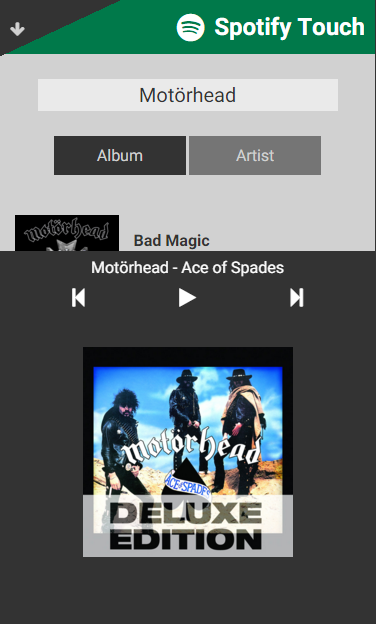
\includegraphics[width=0.9\linewidth]{spotify_now_playing.png}
        \caption{Now Playing view}
        \label{fig:NowPlayingView}
    \end{subfigure}
    \begin{subfigure}{0.45\columnwidth}
        \centering
        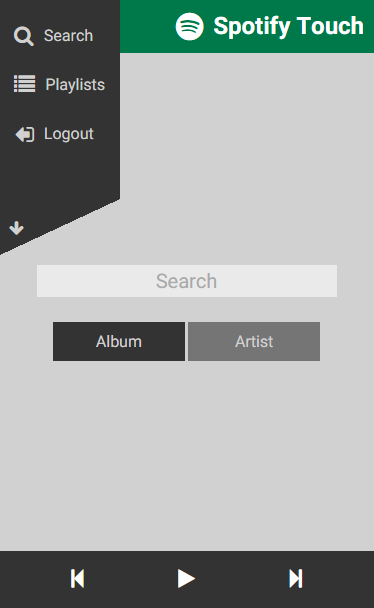
\includegraphics[width=0.9\linewidth]{spotify_menu.png}
        \caption{Main menu open}
        \label{fig:MenuView}
    \end{subfigure}
    \caption{User interface on a mobile display.}
    \label{fig:GUI}
\end{figure}

Figure \ref{fig:GUI} shows different views of the application.
The default view after logging in is the search view shown in figure \ref{fig:SearchView}.
The search view allows the user to search for either music albums or artists.
Typing text in the search term field automatically triggers the search and shows results as a list below.
The list can be scrolled up and down by dragging with one finger.

Figure \ref{fig:PlaylistView} shows the playlist view, where the user can view, edit and listen to their playlists.
\todo[inline]{Kuvaus playlistien eri touch eventeista.}

The currently playing track is always visible on the bottom of the screen.
By dragging the bottom bar up, the album cover art becomes visible, as shown in figure \ref{fig:NowPlayingView}.
The next or previous track can be played by swiping the cover art image left or right.

A menu tab is always visible in the top left corner of the display.
Dragging the tab down with one finger opens the menu, as shown in figure \ref{fig:MenuView}.
The menu lets the user select either the search view or the playlist view, or log out completely.
The menu can be closed by dragging the tab back up.

\begin{table}[htbp]
    \centering
    \begin{tabular}{|l | c | c | c | c |}
        \hline
         Gesture & Menu & Search & Playlists & Now Playing \\ \hline
         Swipe &   &   & x & x \\ \hline
         Drag  & x & x & x & x \\ \hline
         Hold  &   &   & x &   \\ \hline
    \end{tabular}
    \caption{Gestures used in different views}
    \label{tab:Gestures}
\end{table}

Altogether three different touch gestures are used in the user interface.
The gestures are summarized in table \ref{tab:Gestures}.


\section{Research methods}
\todo[inline]{Toimivuuden arvioinnista.}

\section{Results}

\begin{table}[htbp]
    \centering
    \begin{tabular}{| l | c | p{4cm} |}
        \hline
        Device & Browser & Notes \\ \hline
        Windows PC & Chrome & Touch emulation seems to stop working from time to time. \\ \hline
        Sony Xperia Z3 & Chrome & Works similar to desktop Chrome. Search results get unintentionally scrolled from time to time. \\ \hline
        Nokia Lumia 1520 & Internet Explorer & Dragging and swiping does not work at all. \\ \hline
    \end{tabular}
    \caption{Tested devices}
    \label{tab:devices}
\end{table}

We collected feedback from user tests.
A summary of the most common comments is shown below.

\begin{itemize}
    \item Tap-and-hold gesture unintuitive without any visual feedback, and easy to do unintentionally.
    \item Search result list might get scrolled when the user drags or swipes another element in front of the list.
\end{itemize}

\section{Analysis}
...

\section{Conclusions}
...





% if have a single appendix:
%\appendix[Proof of the Zonklar Equations]
% or
%\appendix  % for no appendix heading
% do not use \section anymore after \appendix, only \section*
% is possibly needed

% use appendices with more than one appendix
% then use \section to start each appendix
% you must declare a \section before using any
% \subsection or using \label (\appendices by itself
% starts a section numbered zero.)
%


%\appendices
%\section{Proof of the First Zonklar Equation}
%\blindtext

% use section* for acknowledgement
%\section*{Acknowledgment}


%The authors would like to thank...


% Can use something like this to put references on a page
% by themselves when using endfloat and the captionsoff option.
\ifCLASSOPTIONcaptionsoff
  \newpage
\fi



% trigger a \newpage just before the given reference
% number - used to balance the columns on the last page
% adjust value as needed - may need to be readjusted if
% the document is modified later
%\IEEEtriggeratref{8}
% The "triggered" command can be changed if desired:
%\IEEEtriggercmd{\enlargethispage{-5in}}

% references section

% can use a bibliography generated by BibTeX as a .bbl file
% BibTeX documentation can be easily obtained at:
% http://www.ctan.org/tex-archive/biblio/bibtex/contrib/doc/
% The IEEEtran BibTeX style support page is at:
% http://www.michaelshell.org/tex/ieeetran/bibtex/
%\bibliographystyle{IEEEtran}
% argument is your BibTeX string definitions and bibliography database(s)
%\bibliography{IEEEabrv,../bib/paper}
%
% <OR> manually copy in the resultant .bbl file
% set second argument of \begin to the number of references
% (used to reserve space for the reference number labels box)
\begin{thebibliography}{1}

%\bibitem{IEEEhowto:kopka}
%H.~Kopka and P.~W. Daly, \emph{A Guide to \LaTeX}, 3rd~ed.\hskip 1em plus
  %0.5em minus 0.4em\relax Harlow, England: Addison-Wesley, 1999.
\bibitem{MobileHTML5}
Mobilehtml5.org. 2015. ``Mobile HTML5 compatibility on iPhone, Android, Windows Phone, BlackBerry, Firefox OS and other mobile devices``. [ONLINE] Available at: \url{http://mobilehtml5.org} . [Accessed 23 December 2015].

\bibitem{SpotifyAPI}
Spotify AB. 2015. ``Spotify Web API - Spotify Developer''. [ONLINE] Available at: \url{https://developer.spotify.com/web-api/} . [Accessed 11 October 2015].

\bibitem{HammerJS}
J. Tangelder. 2015. ``Hammer.js - Add touch gestures to your page''. [ONLINE] Available at: \url{http://hammerjs.github.io/} . [Accessed 11 October 2015].

\bibitem{BillinghurstGestures}
S. S. Billinghurst and K. L. Vu, ``Touch screen gestures for web browsing tasks'' in Computers in Human Behaviour, Vol. 53, Dec. 2015, pp. 71-81, 2015.

\bibitem{AngularJS}
AngularJS. 2015. AngularJS - Superheroic JavaScript MVW Framework. [Online] Available at: \url{https://angularjs.org/} . [Accessed 12 October 2015].

\bibitem{BragdonExperimental}
A. Bragdon, E. Nelson, Y. Li, and K. Hinckley, ``Experimental analysis of touch-screen gesture designs in mobile environments'' In Proceedings of the SIGCHI Conference on Human Factors in Computing Systems (CHI '11), 2011.

\bibitem{W3CTouchEvents}
World Wide Web Consortium W3C. 2015. ``Touch Events''. [ONLINE] Available at: \url{http://www.w3.org/TR/touch-events/} . [Accessed 26 December 2015].

\bibitem{W3Counter}
W3Counter. 2015. ``W3Counter: Browser, OS Market Share Trends''. [ONLINE] Available at: \url{http://www.w3counter.com/trends} . [Accessed 27 December 2015].

\bibitem{AndroidMarketShare}
Gartner. 2015. ``Gartner Says Smartphone Sales Surpassed One Billion Units in 2014''. [ONLINE] Available at: \url{http://www.gartner.com/newsroom/id/2996817} . [Accessed 27 December 2015].

\bibitem{GestureVideoPlayer}
S. Buchinger, E. Hotop, H. Hlavacs, F. De Simone, and T. Ebrahimi. 2010. ``Gesture and touch controlled video player interface for mobile devices.'' in Proceedings of the 18th ACM international conference on Multimedia (MM '10).


\end{thebibliography}

% biography section
% 
% If you have an EPS/PDF photo (graphicx package needed) extra braces are
% needed around the contents of the optional argument to biography to prevent
% the LaTeX parser from getting confused when it sees the complicated
% \includegraphics command within an optional argument. (You could create
% your own custom macro containing the \includegraphics command to make things
% simpler here.)
%\begin{biography}[{\includegraphics[width=1in,height=1.25in,clip,keepaspectratio]{mshell}}]{Michael Shell}
% or if you just want to reserve a space for a photo:

\begin{IEEEbiography}[{\includegraphics[width=1in,height=1.25in,clip,keepaspectratio]{picture}}]{John Doe}
\blindtext
\end{IEEEbiography}

% You can push biographies down or up by placing
% a \vfill before or after them. The appropriate
% use of \vfill depends on what kind of text is
% on the last page and whether or not the columns
% are being equalized.

%\vfill

% Can be used to pull up biographies so that the bottom of the last one
% is flush with the other column.
%\enlargethispage{-5in}




% that's all folks
\end{document}


